% C6. Escalera del error
\begin{frame}{Cada idea, cuánto bajó el error: los datos importaron más que el algoritmo}
  \centering
  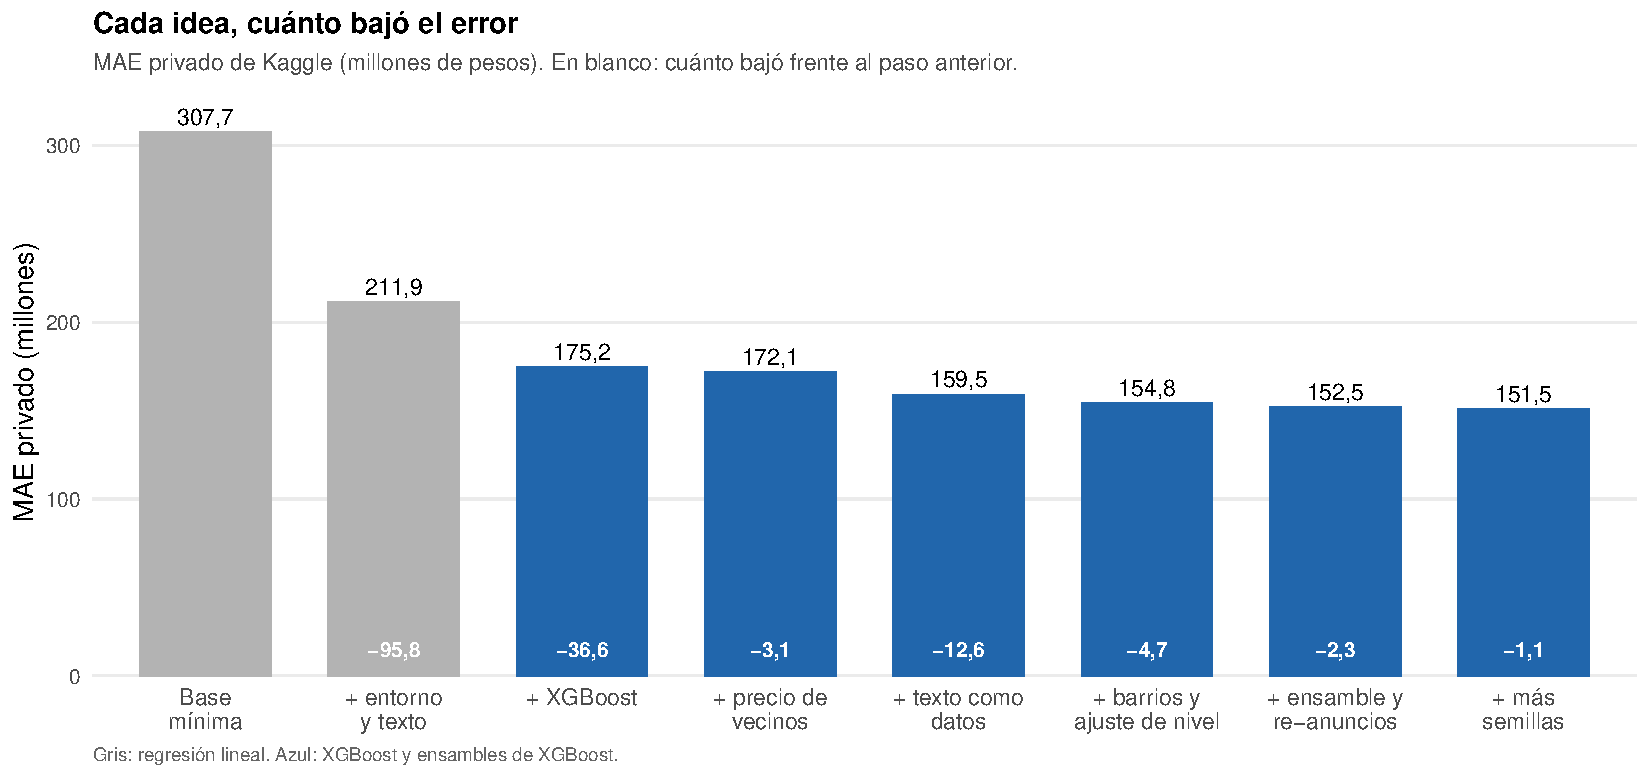
\includegraphics[width=\textwidth]{pres_escalera.pdf}
  \note{Pasar de una base mínima a la base con entorno y texto bajó el error \pasoentorno{} millones. Cambiar la regresión lineal por XGBoost, \pasoxgb{} millones. Después, el texto como datos fue el salto más grande (\pasotexto{} millones). El ensamble, los modelos del precio por m$^2$, las semillas y el ajuste de nivel aportan menos, pero suman. Los embeddings del último paso casi no recibieron peso en el ensamble.}
\end{frame}
